\title{Informe de Estadística en Física Experimental: Ejercicio 13 de la guia 8,  13 y 14 de la  Guía 9}
\author{Andrés Babino}

\begin{document}
\maketitle
\section{Introducción}
El lenguaje utilizado para programar todas los ítems fue Python.
El código utilizado para generar los datos, gráficos y este mismo informe fue controlado con git, tiene licencia MIT y está almacenado en \url{https://github.com/ababino/efe}.

\section*{Guía 8, Ejercicio 13, ítem a}
Como las mediciones son a tiempo fijo la variable aleatoria es poissonian.
Si se desea ajustar la curva $y(t) = a_1 + a_2 e^{-t/209.69s} + a_3 e^{-t/34.244s}$ a un conjunto de datos se deben usar las fórmulas de cuadrados mínimos lineal.
Los parámetros quedan determinados por:
$$
\vec{\theta} = (AV^{-1}A)^{-1}AV^{-1}y
$$
Donde $\theta$ es el vetor de parametros $(a_1, a_2, a_3)$ y $A$ es una matriz que tiene unos en la primera columna $e^{-t/209.69s}$, en la segunda y $e^{-t/34.244s}$ en la tercera.
$V$ es la matriz de covarianza de la variable independiente.
En este caso la matriz es diagonal porque los datos no están correlacionados y la varianza es poisson.

La matriz de covarianza de los parámetros ajustados se puede calcular de la siguiente manera:
$$
Cov(\vec{\theta}) = (AV^{-1}A)^{-1}
$$
Los resultados de este ajuste fueron:
$$
\vec{\theta} = (10.1, 128, 960)
$$
$$
V(\vec{\theta}) =\left(
\begin{matrix}
0.70 &-3.3 & 7.0 \\
-3.3 & 38 &-99 \\
7.0  & -99 & 100
\end{matrix} \right)
$$

Usando estos datos podemos calcular el valor esperado del cociente $a_2/a_3$ y usando la fórmula de propagacón de errores su error:

$$
\frac{a_2}{a_3} = 0.134 \pm 0.050
$$

\section*{Guía 8, Ejercicio 13, ítem b}
Si $a_4$ y $a_5$ son desconocidos la función a ajustar no es lineal en los parámetros.
Linealizando la función $\chi^2$ con respecto a los parámetros obtenemos:
$$
\vec{\theta}=(10\ 128\ 957\  210\  34)
$$
$$
Cov(\vec{\theta}) = \left(
\begin{matrix}
4.0 & 34 &  0.44 & -61 & -3.1\\
34 & 530 & 150  -74 & -53\\
0.44 & 150 & 2600 & -98 & -79\\
-61 & -740 & -98 & 1200 & 69\\
-3.1 & -53 & -79 & 69. & 7.5
\end{matrix}
\right)
$$
\section*{Guía 8, Ejercicio 13, ítem c}
En este caso la función $chi^2$ es:
$$
t(a_1, a_2, a_3, a_4, a_5) = \sum_{i=1}^N \frac{\left(y_i-a_1 - a_2 e^{-t/a_4} - a_3 e^{-t/a_5}\right)^2}{y_i}
$$
que debido a que los parámetros $a_4$ y $a_5$ están en las exponenciales el $chi^2$ no es cuadrático en los parámetros.

Si en el argumento de t dejamos fijo $a_1=a_1*$, $a_2=a_2*$ y $a_3=a_3*$ los valore óptimos ya calculados obtenomos una función de $a_4$ y $a_5$.
 Otra opción es para cada par $(a_4, a_5)$ calcular la terna óptima $(a_1, a_2, a_3)$ y con ellos calcular el $chi^2$.
 En el gráfico de la figura \ref{fig:fig1} se muestra la curva de nivel $t=t_{min} + 1$ para las dos funciones.

\begin{figure}
\centering
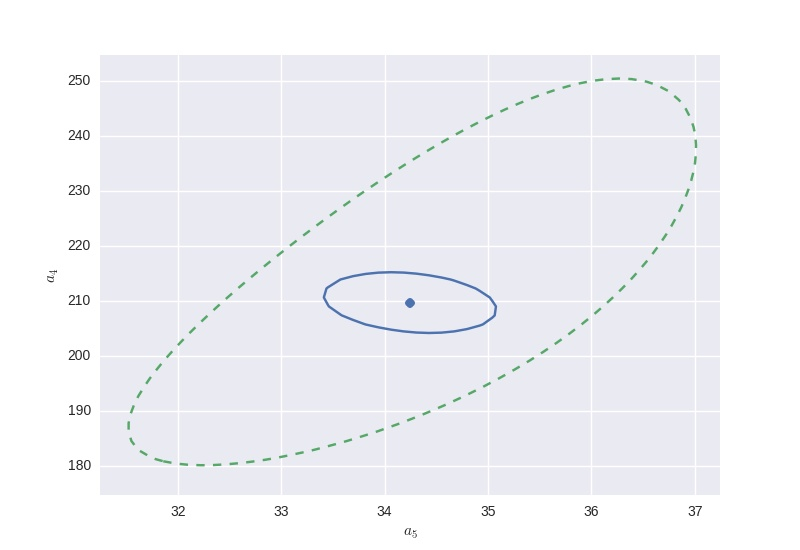
\includegraphics[width=0.75\textwidth]{fig1.jpg}
\caption[]{}
\label{fig:fig1}
\end{figure}


\section*{Guía 9}
\subsection*{Ejercicio 13}
\subsubsection*{Ítem a}
Por simple inspección ocular se pueden ordenar los histogramas como se muestra en la figura \ref{fig:hists}
\begin{figure}
\centering
\begin{subfigure}[b]{0.3\textwidth}
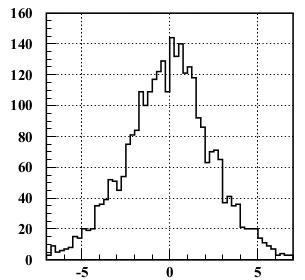
\includegraphics[width=0.84\textwidth]{hist3.jpg}
\end{subfigure}
\begin{subfigure}[b]{0.3\textwidth}
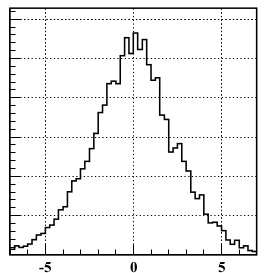
\includegraphics[width=0.75\textwidth]{hist2.jpg}
\end{subfigure}
\begin{subfigure}[b]{0.3\textwidth}
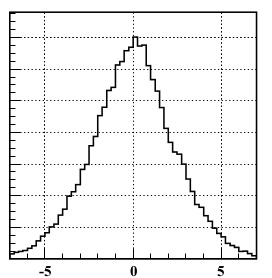
\includegraphics[width=0.75\textwidth]{hist1.jpg}
\end{subfigure}
\caption[]{}
\label{fig:hists}
\end{figure}

\subsubsection*{Ítem b}
En la figura \ref{fig:fig2} se muestra un histograma de los primeros $3000$ datos.
Sobre estos se graficó las cuentas esperadas asumiendo una distribución N(0, 2.5).
Si aplicamos un test $chi^2$ sobre estos datos obtenemos que un valor $chi^2 =chi2=67$.
El número de grados de libertad de la $chi^2$ es $56$ (el número de bines) por lo tanto el p valor del test es $pval=0.15$

\begin{figure}
\centering
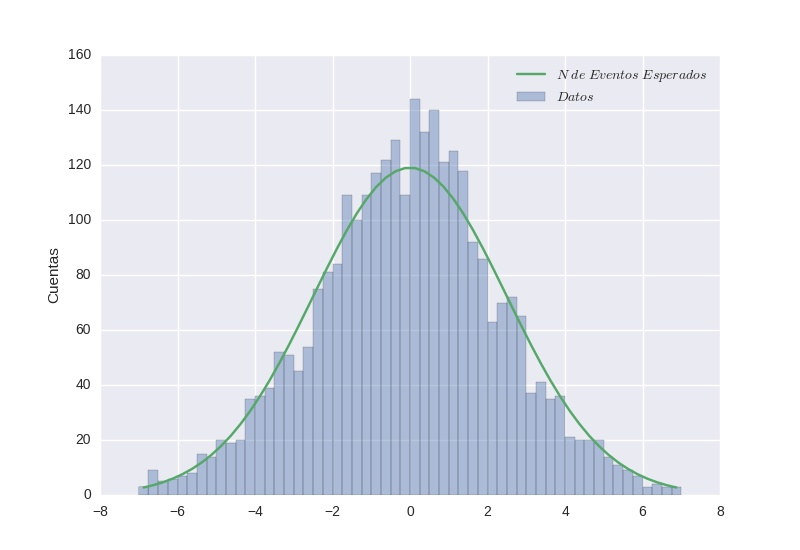
\includegraphics[width=0.75\textwidth]{fig2.jpg}
\caption[]{}
\label{fig:fig2}
\end{figure}
